\documentclass[../../Main.tex]{subfiles}

\begin{document}
    \begin{figure}[hbt!]
        \centerline{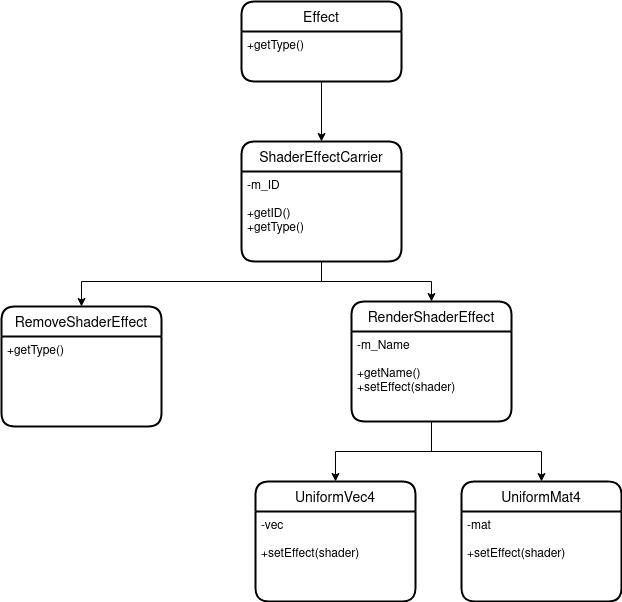
\includegraphics[scale=0.5]{img/Classes/Effects.png}}
        \caption{Effect subclasses}
        \label{fig}
    \end{figure}
    Effect
    \begin{center}
        Functions
        \begin{tabular}{ | m{0.15\textwidth} | m{0.35\textwidth}| m{0.4\textwidth} | }
            \hline
            \textbf{Function Name} & \textbf{Parameters} & \textbf{Description} \\
            \hline
            getType & & Returns the type of the effect \\
            \hline
        \end{tabular}
    \end{center}
    ShaderEffectCarrier
    \begin{center}
        Variables
        \begin{tabular}{ | m{0.45\textwidth} | m{0.45\textwidth} | }
            \hline
            \textbf{Variable Name} & \textbf{Description} \\
            \hline
            m\_ID & Stores the ID of the effect \\
            \hline
        \end{tabular}
        Functions
        \begin{tabular}{ | m{0.15\textwidth} | m{0.35\textwidth}| m{0.4\textwidth} | }
            \hline
            \textbf{Function Name} & \textbf{Parameters} & \textbf{Description} \\
            \hline
            getID & & Returns the ID of the effect \\
            \hline
        \end{tabular}
    \end{center}
    RemoveShaderEffect - Inherits everything from parent classes and only overrides \\
    ShaderEffect
    \begin{center}
        Variables
        \begin{tabular}{ | m{0.45\textwidth} | m{0.45\textwidth} | }
            \hline
            \textbf{Variable Name} & \textbf{Description} \\
            \hline
            m\_Name & Stores the name of the variable \\
            \hline
        \end{tabular}
        Functions
        \begin{tabular}{ | m{0.15\textwidth} | m{0.35\textwidth}| m{0.4\textwidth} | }
            \hline
            \textbf{Function Name} & \textbf{Parameters} & \textbf{Description} \\
            \hline
            getName & & Returns the name of the variable \\
            \hline
            setEffect & shader to set the effect to & Sets the current effect to the shader given \\
            \hline
        \end{tabular}
    \end{center}
    UniformVec4
    \begin{center}
        Variables
        \begin{tabular}{ | m{0.45\textwidth} | m{0.45\textwidth} | }
            \hline
            \textbf{Variable Name} & \textbf{Description} \\
            \hline
            vec & Stores the vector that is passed into the shader \\
            \hline
        \end{tabular}
    \end{center}
    UniformMat4
    \begin{center}
        Variables
        \begin{tabular}{ | m{0.45\textwidth} | m{0.45\textwidth} | }
            \hline
            \textbf{Variable Name} & \textbf{Description} \\
            \hline
            mat & Stores the matrix that is passed into the shader \\
            \hline
        \end{tabular}
    \end{center}
\end{document}